\chapter{Project Analysis} %TODO

\section{Problem definition}

\paragraph{}
Today, the health data that we can access through the internet is quite large. However, due to the data pollution in this area, people may think that they are	caught	in	a	deadly	illness when	they	search	for	a	complaint	they	are	experiencing	on	the	internet.	Even	diseases	that require	long-term	examination	and	detailed	analysis	to	be	diagnosed	can	easily	be	presented to	people.	What's	more,	there	are	many	forums	that	bring	doctors	and	people	together	on	the	internet,	as	well	as	sites	that	function	as	an	individual	dialogue.	On	these	pages,	people	can	ask	irrelevant	or	absurd	questions	to	doctors	because	of	wrong	information	or	ignorance. 

\section{Problem solution}

\paragraph{}
Bot is asking for first symptoms \\
Written language recognition \\
Determine symptoms \\
Compute first set of diseases \\
Ask directed questions to reduce the set \\
Continue until the set is small enough \\
Gives results along with advices 

\section{Decision Support System}

\paragraph{}
Interactive and easy to use \\
Knowledge-driven DSS

\paragraph{}
Input: symptoms + personal data \\
Output: 3 most probable diseases and advices \\
Limited by the database \\
Compute probability on diseases depending input data \\
Takes decision when threshold reached \\
Maximum number of questions \\
Maximum probability 


\section{SWOT Analysis}

\begin{figure}[H]
	\centering
	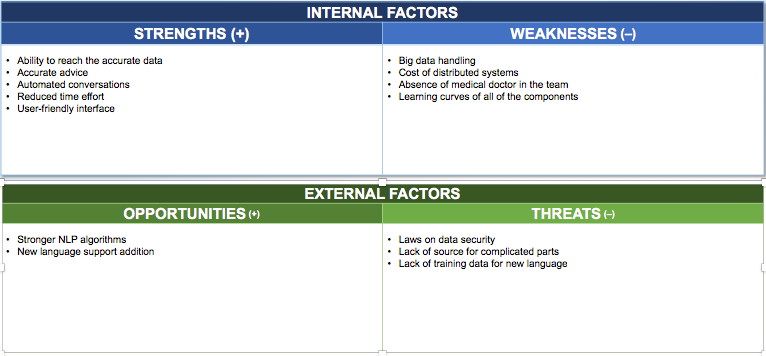
\includegraphics[width=\textwidth]{swot}
	\caption{SWOT Analysis}
	\label{swot}
\end{figure}

\section{Division of labor}

We did not have an experience in the chatbot field, and because of our lack of experience in python	tools, we did the work part in accordance with the principle of volunteering. In this context we divided the different tasks as showed on table \ref{labor}.
\begin{table}[H]
	\centering
	\begin{tabular}{|c|p{10cm}|}
		\hline
		\textbf{Group member} & \textbf{Labor} \\
		\hline
		Emirhan	Kutlu & Django back-end, ChatterBot usage and integration, Telegram chat bot programming and competitive and SWOT Analysis \\
		\hline
		Lucie Labadie & Django back-end, Multi-classifier with SciKit-learn and documentation, supervision report \\
		\hline
		Rosen Sasav & Public database search, Database architectural design and front-end \\
		\hline
	\end{tabular}
	\caption{Division of labor}
	\label{labor}
\end{table}	

Apart from these, collaborated studies and meetings	were held to decide on the method needed for diagnosis.